
\section{Placement}
\label{sec:placement}
So far we have only dealt with technology problems where we consider the problem space and adress the constraints of the hardware architecture. 
For every constraint, we devise a solution to fully address it or a simplification that sacrifices some optimization but reduces the complexity of the problem space. 

Now that we have dealt with the bulk of these constraints and squared them away into self-contained \texttt{SiteInst}s, we can now more easily apply some general optimization algorithms to finally address our optimization objective, which is to place these \texttt{SiteInst} objects onto the device while minimizing wirelength. 

\subsection{Simulated Annealing}
\label{subsec:simulated_annealing}

In this paper we implement and present a basic Simulated Annealing (SA) placer. 
As mentioned in the Introduction, SA is a metaheuristic that approximates a global optimum in a large optimization search space. 
SA does not guarantee a globally optimal solution, but provides solutions that are often "good enough", especially when finding an approximate global optimum is more important than finding a precise local optimum in a fixed amount of time. 
SA is typically employed in discrete combinatorial optimization problems like the travelling salesman problem or job-shop scheduling. 
It is directly inspired by Annealing in metallurgy, which is the physical process of heating a metal above its crystallization temperature, allowing its atoms to migrate through the crystal lattice, and slowly cooling it to allow its atoms to recrystallize into a more desirable structure, such as one that minimizes structural defects. 

The state \(s\) of the system and the function \(E(s)\) to be minimized is analogous to the internal energy of the system. 
In metallurgic Annealing, the state \(s\) represents the position of every atom in the metal object at any given snapshot in time, while \(E(s)\) represents the defectiveness in the metal's structure however that may be quantified. 
In the context of our SA placer, the state \(s\) represents the placement of every \texttt{SiteInst} on the \texttt{device} at any given iteration, while \(E(s)\) represents the total wirelength of \texttt{Net}s between all \texttt{SiteInst}s of the current placement.
We will be measuring wirelength using the manhattan distance between the 2-dimensional coordinates of the \texttt{SiteInst}s on the \texttt{device}.
We will refer to these distances as half perimeter wirelength (HPWL).
The goal of SA is to bring the system from some initial state to a state with lower energy until some stopping criterion is met, whether that be when a computational budget is exceeded, an energy budget is met, or until the energy's rate of change approaches zero. 

At each step or iteration, the algorithm considers some neighboring state \(s^*\). 
If \(s^*\) has a lower energy than \(s\), then the state transition from \(s\) to \(s^*\) is accepted outright.
If \(s^*\) has a higher energy, then it can probabilistically be accepted depending on the current global temperature.
The higher the temperature, the higher the likelihood of accepting an energy-increasing move. 
The global temperature starts at some positive amount then gradually decreases to zero according to a cooling schedule.
This cooling schedule can be linear, geometric, logarithmic, or some piecewise combination. 
Its parameters can be fine tuned through empirical experimentation. 

Shown in Listing \ref{lst:sa_outer} is a simplified pseudocode for the outer-most loop of our placer's SA algorithm. 
First, we randomly place all \texttt{SiteInst}s across the \texttt{device}.
Then, we initialize a simple geometric cooling schedule: 
\begin{equation}
    \label{coolingSchedule}
    T_{n+1} = \alpha T_n
\end{equation}
with initial temperature \(T_0=10000\), cooling rate \(\alpha=0.98\), and \(n = \{0, 1, 2, ..., 300\}\) passes.
Hill-climbing moves can be accepted via the probability function \(P()\): 
\begin{equation}
    \label{moveAcceptance}
    P(s, s^*, T_n) = exp(\frac{E(s) - E(s^*)}{T_n})
\end{equation}
where \(E(s^*)\) is the energy of the proposed state \(s^*\), \(E(s)\) is the energy of the current state \(s\), and \(T_n\) is the current global temperature at \(n\) passes. 
If \(P(s, s^*, T_n) < random(0, 1)\), then \(s \leftarrow s^*\).
Recall that this probability is only evaluated for hill-climbing moves, thus the cost difference \(E(s) - E(s^*)\) is always negative.
In summary, a lower cost difference and a higher temperature contributes to a higher probabilty of hill-climbing acceptance.
All hill-descending moves on the other hand are simply accepted outright. 

Then, we enter the outer-most loop which terminates when the number of passes exceeds our computational budget, in this case, 300 passes. 
In each pass, we \texttt{moveAll()} the design, then update the global temperature. 

In each \texttt{moveAll()}, we iterate through four mutually exclusive groups of placement objects: \texttt{DSPSiteInstCascades}, \texttt{CARRYSiteInstChains}, \texttt{RAMSiteInst}s, and \texttt{CLBSiteInst}s (single SLICEs that do not belong to CARRY chains).
For each placement object in the pass, we propose a new placement for that object on the device. 
Each proposed movement represents a proposed state transition of system. 
If the design has for example, 50 \texttt{DSPSiteInstCascades}, 100 \texttt{CARRYSiteInstChains}, 75 \texttt{RAMSiteInst}s, and 250 \texttt{CLBSiteInst}s, and we set a budget of 300 passses, then the algorithm will consider up to \(300 * (50 + 100 + 75 + 250) = 142500\) state transitions. 
If the proposed \texttt{Site} is already occupied by a resident or existing \texttt{SiteInst}, we evaluate a swap in their placements. 

In SA, proposed movements are selected randomly, then accepted or rejected based on legality and cost. 
Figure \ref{fig:swapSingleSite} shows how a swap proposal between singular \texttt{CLBSiteInst}s or between \texttt{RAMSiteInst}s is evaluated, while Listing \ref{lst:sa_move_single} shows the corresponding Java code.
On the other hand, the movement of \texttt{SiteInst} chains is considerably more complex because there are more placement constraints to consider, especially when swapping the positions between multiple chains.
Figure \ref{fig:swapSiteChain} shows a demonstration of how two \texttt{DSPSiteInstCascades} or two \texttt{CARRYSiteInstChains} can be swapped while Listing \ref{lst:chain_swap_pseudocode} shows the corresponding pseudocode. 

In more sophisticated placers, the proposed movement can also be selected by finding the centroid between \texttt{SiteInst}s that share a net with the current object, or even a hybrid of random and centroid selection. 
Moves that actively attempt to predict a better placement are often referred to as "directed" moves in literature. 
Placers that take inspiration from physical interactions like gravity or electrostatics are often referred to as "force directed" placers and are akin to physics simulators. 

Directed moves as opposed to undirected moves give rise to the concept of legalization. 
When using undirected moves as in SA, we can simply keep track of a \texttt{List} or \texttt{HashMap} of occupied \texttt{Site}s and available \texttt{Site}s and select from that data structure via random selection. 
However, for directed moves like centroid selection, the centroid between \texttt{Site}s may not necessarily fall directly on another discrete \texttt{Site} on the \texttt{device}. 
Even when it does, the centroid \texttt{Site} may be incompatible with the \texttt{SiteInst} or may fail to meet some other placement constraint. 
In such cases, we must do a neighborhood search around the centroid up to a certain radius to find a \texttt{Site} that satisfies all the constraints of the \texttt{SiteInst} at hand. 
We will take some inspiration from ray-marching in graphics and do a diamond-shaped spiral search around the centroid where we check the legality of each \texttt{Site} as we step through the spiral and select the first \texttt{Site} that meets all of the placement constraints. 

In force directed placers, there is a concept of global placement followed by detailed placement
Global placement places objects freely on an analog plane and is driven by directed movement or analytical solution.
In global placement, objects do not have to adhere to any hardware constraints and can even overlap with one another.
Detailed placement takes the global placement and attempts to fit it within the constraints of the hardware. 
Detailed placement "legalize" the global placement by discretizing the analog positions of the objects onto the discrete grid of resources of the \texttt{device}.
Overlapping objects are spread out until every \texttt{SiteInst}-\texttt{Cell} is assigned its own unique \texttt{Site}-\texttt{BEL}.

There also exists other strategies to mix packing, placement, and legalization in different ways. (CITE THAT ONE PAPER).
In this context, our placer follows a straightforward pack-legalize-place strategy. 

If the move reduces the HPWL cost, then the movement is accepted outright.
If the move increases cost, then it can be accepted by chance if the global temperature is high enough to permit the hill-climb.
The temperature decreases with each pass until reaching zero, at which point, the algorithm makes exclusively energy-decreasing moves, effectively reducing into a greedy algorithm. 
The hope is that by this point, the placement has already crystallized into an approximate global optimum and the greediness of the algorithm will help the system settle deeper into the energy well faster. 
We can also switch from random selection to centroid selection when the temperature approaches near zero to speed up the settlement further. 



\newcolumn
\begin{lstlisting}[language=java, caption={SA pseudocode: outer loop}, label={lst:sa_outer}]
public void placeDesign(PackedDesign packedDesign) {
    randomInitialPlacement(packedDesign);
    // init_temp=10000, alpha=0.98, max_passes=300
    initCoolingSchedule(10000, 0.98, 300)
    int passes = 0;
    while (passes < 300) {
        updateTemperature(passes);
        moveAll(packedDesign)
        passes++;
    }
}

private void moveAll(PackedDesign packedDesign) {
    moveSiteChains(packedDesign.DSPSiteInstCascades);
    moveSiteChains(packedDesign.CARRYSiteInstChains);
    moveSingleSite(packedDesign.RAMSiteInsts);
    moveSingleSite(packedDesign.CLBSiteInsts);
}
\end{lstlisting}


\begin{lstlisting}[language=java, caption={Single Site Movement}, label={lst:sa_move_single}]
protected void moveSingleSite(List<SiteInst> sites) {
for (SiteInst si : sites) {
    SiteTypeEnum ste = si.getSiteTypeEnum();
    List<Site> homeConns = findConnectedSites(si, null);
    Site homeSite = si.getSite();
    Site awaySite = proposeSite(si, homeConns, true);
    SiteInst awaySi = occupiedSites.get(ste).get(awaySite);
    double oldCost = 0;
    double newCost = 0;
    if (awaySi != null) {
        List<Site> awayConns = findConnectedSites(awaySi, null);
        oldCost += evaluateSite(homeConns, homeSite);
        oldCost += evaluateSite(awayConns, awaySite);
        newCost += evaluateSite(homeConns, awaySite);
        newCost += evaluateSite(awayConns, homeSite);
    } else {
        oldCost += evaluateSite(homeConns, homeSite);
        newCost += evaluateSite(homeConns, awaySite);
    }
    if (evaluateMoveAcceptance(oldCost, newCost)) {
        if (awaySi != null) {
            unplaceSiteInst(si);
            unplaceSiteInst(awaySi);
            placeSiteInst(si, awaySite);
            placeSiteInst(awaySi, homeSite);
        } else {
            unplaceSiteInst(si);
            placeSiteInst(si, awaySite);
        }
    }
}
} // end randomMoveSingleSite()
\end{lstlisting}

{
    \centering
    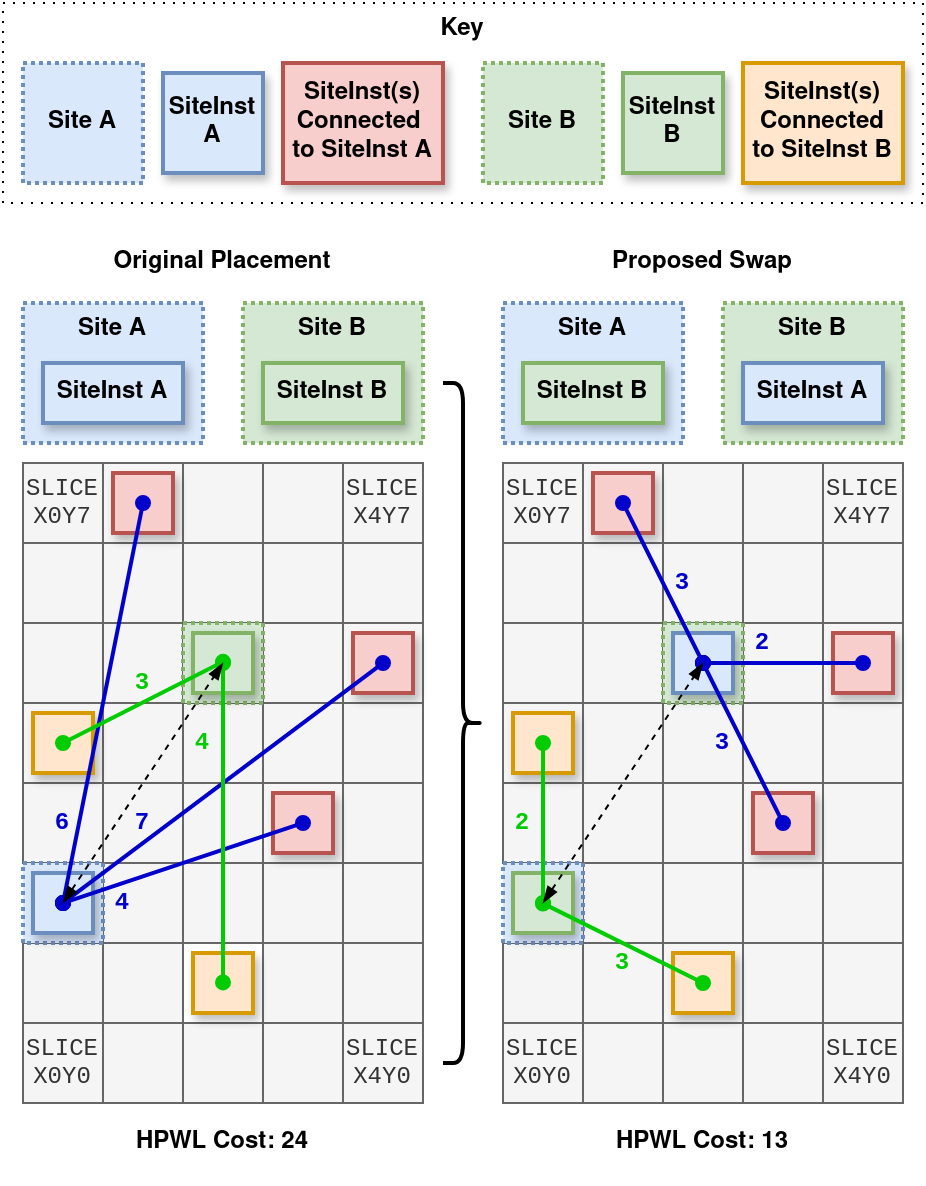
\includegraphics[width=\columnwidth]{figures/placement/swapSingleSite.png}
    \captionof{figure}{Single Site Swap Proposal}
    \label{fig:swapSingleSite}
}
\vfill

\begin{lstlisting}[language=java, caption={Cooling Schedule and Move Acceptance with Temperature}, label={lst:sa_acceptance}]
protected List<Double> coolingSchedule;
public void initCoolingSchedule(double initialTemp, double alpha, int movesLimit) {
    double currentTemp = initialTemp;
    for (int i = 0; i < movesLimit; i++) {
        this.coolingSchedule.add(currentTemp);
        currentTemp *= alpha; // geometric cooling
    }
}

protected boolean evaluateMoveAcceptance(double oldCost, double newCost) {
    // if the new cost is lower, accept it outright
    if (newCost < oldCost)
        return true;
    // otherwise, evaluate probability to accept higher cost
    double delta = newCost - oldCost;
    double acceptanceProbability = 
        Math.exp(-delta / this.currentTemp);
    return Math.random() < acceptanceProbability;
}
\end{lstlisting}

\begin{lstlisting}[language=Java, caption={Chain Swapping Pseudocode}, label={lst:chain_swap_pseudocode}]
protected void moveSiteChains(List<List<SiteInst>> chains) {
for (List<SiteInst> currentChain : chains) {
    int chainSize = currentChain.size();

    // Step 1: Identify home window for this chain
    Site homeAnchor = currentChain.get(0).getSite();
    List<Site> homeWindow = getSitesInWindow(homeAnchor, chainSize);

    // Step 2: Select a candidate away anchor
    Site awayAnchor = proposeAnchorSite(currentChain, homeWindow, true);

    // Step 3: Determine away window based on awayAnchor and chainSize
    List<Site> awayWindow = getSitesInWindow(awayAnchor, chainSize);

    // Step 4: Find any resident SiteInst chains in the away window
    List<List<SiteInst>> residentChainsInAway = 
        collectChainsInWindow(siteType, awayWindow);

    // Step 5: If any resident chains overlap with the away window, extend the away window to fully accomodate them 
    if (!residentChainsInAway.isEmpty()) {
        awayWindow = extendWindowToIncludeChains(awayWindow, residentChainsInAway);
    }

    // Step 6: Map the (possibly extended) away window back onto the original region so that the tail of that window coincides with the tail of the current chain
    List<Site> candidateHomeWindow = mapAwayToHomeWindow(
        homeAnchor, awayWindow, chainSize);

    // Step 7: While the candidate home window still overlaps resident chains, shift upward
    int shifts = 0;
    while (windowHasOverlap(candidateHomeWindow)) {
        candidateHomeWindow = shiftWindowUp(candidateHomeWindow);
        shifts++;
        if (shifts > (homeWindow.size() - chainSize)) {
            // Reject this swap attempt.
            // Move on to the next chain.
            continue;
        }
    }

    // Step 8: Compute cost of the original placement in home window
    double oldCost = evaluateWindowCost(homeWindow);

    // Step 9: Compute cost of the proposed swap placement
    double newCost = evaluateWindowCostForSwap(
        homeWindow, awayWindow, currentChain);

    // Step 10: Decide whether to accept the move based on oldCost, newCost, and temperature
    if (evaluateMoveAcceptance(oldCost, newCost, currentTemp)) {
        // Step 11: Perform an element-wise swap of SiteInsts between homeWindow and awayWindow
        swapChainsBetweenWindows(homeWindow, awayWindow);
    }
}
}
\end{lstlisting}


\newpage
\end{multicols}
{
    \centering
    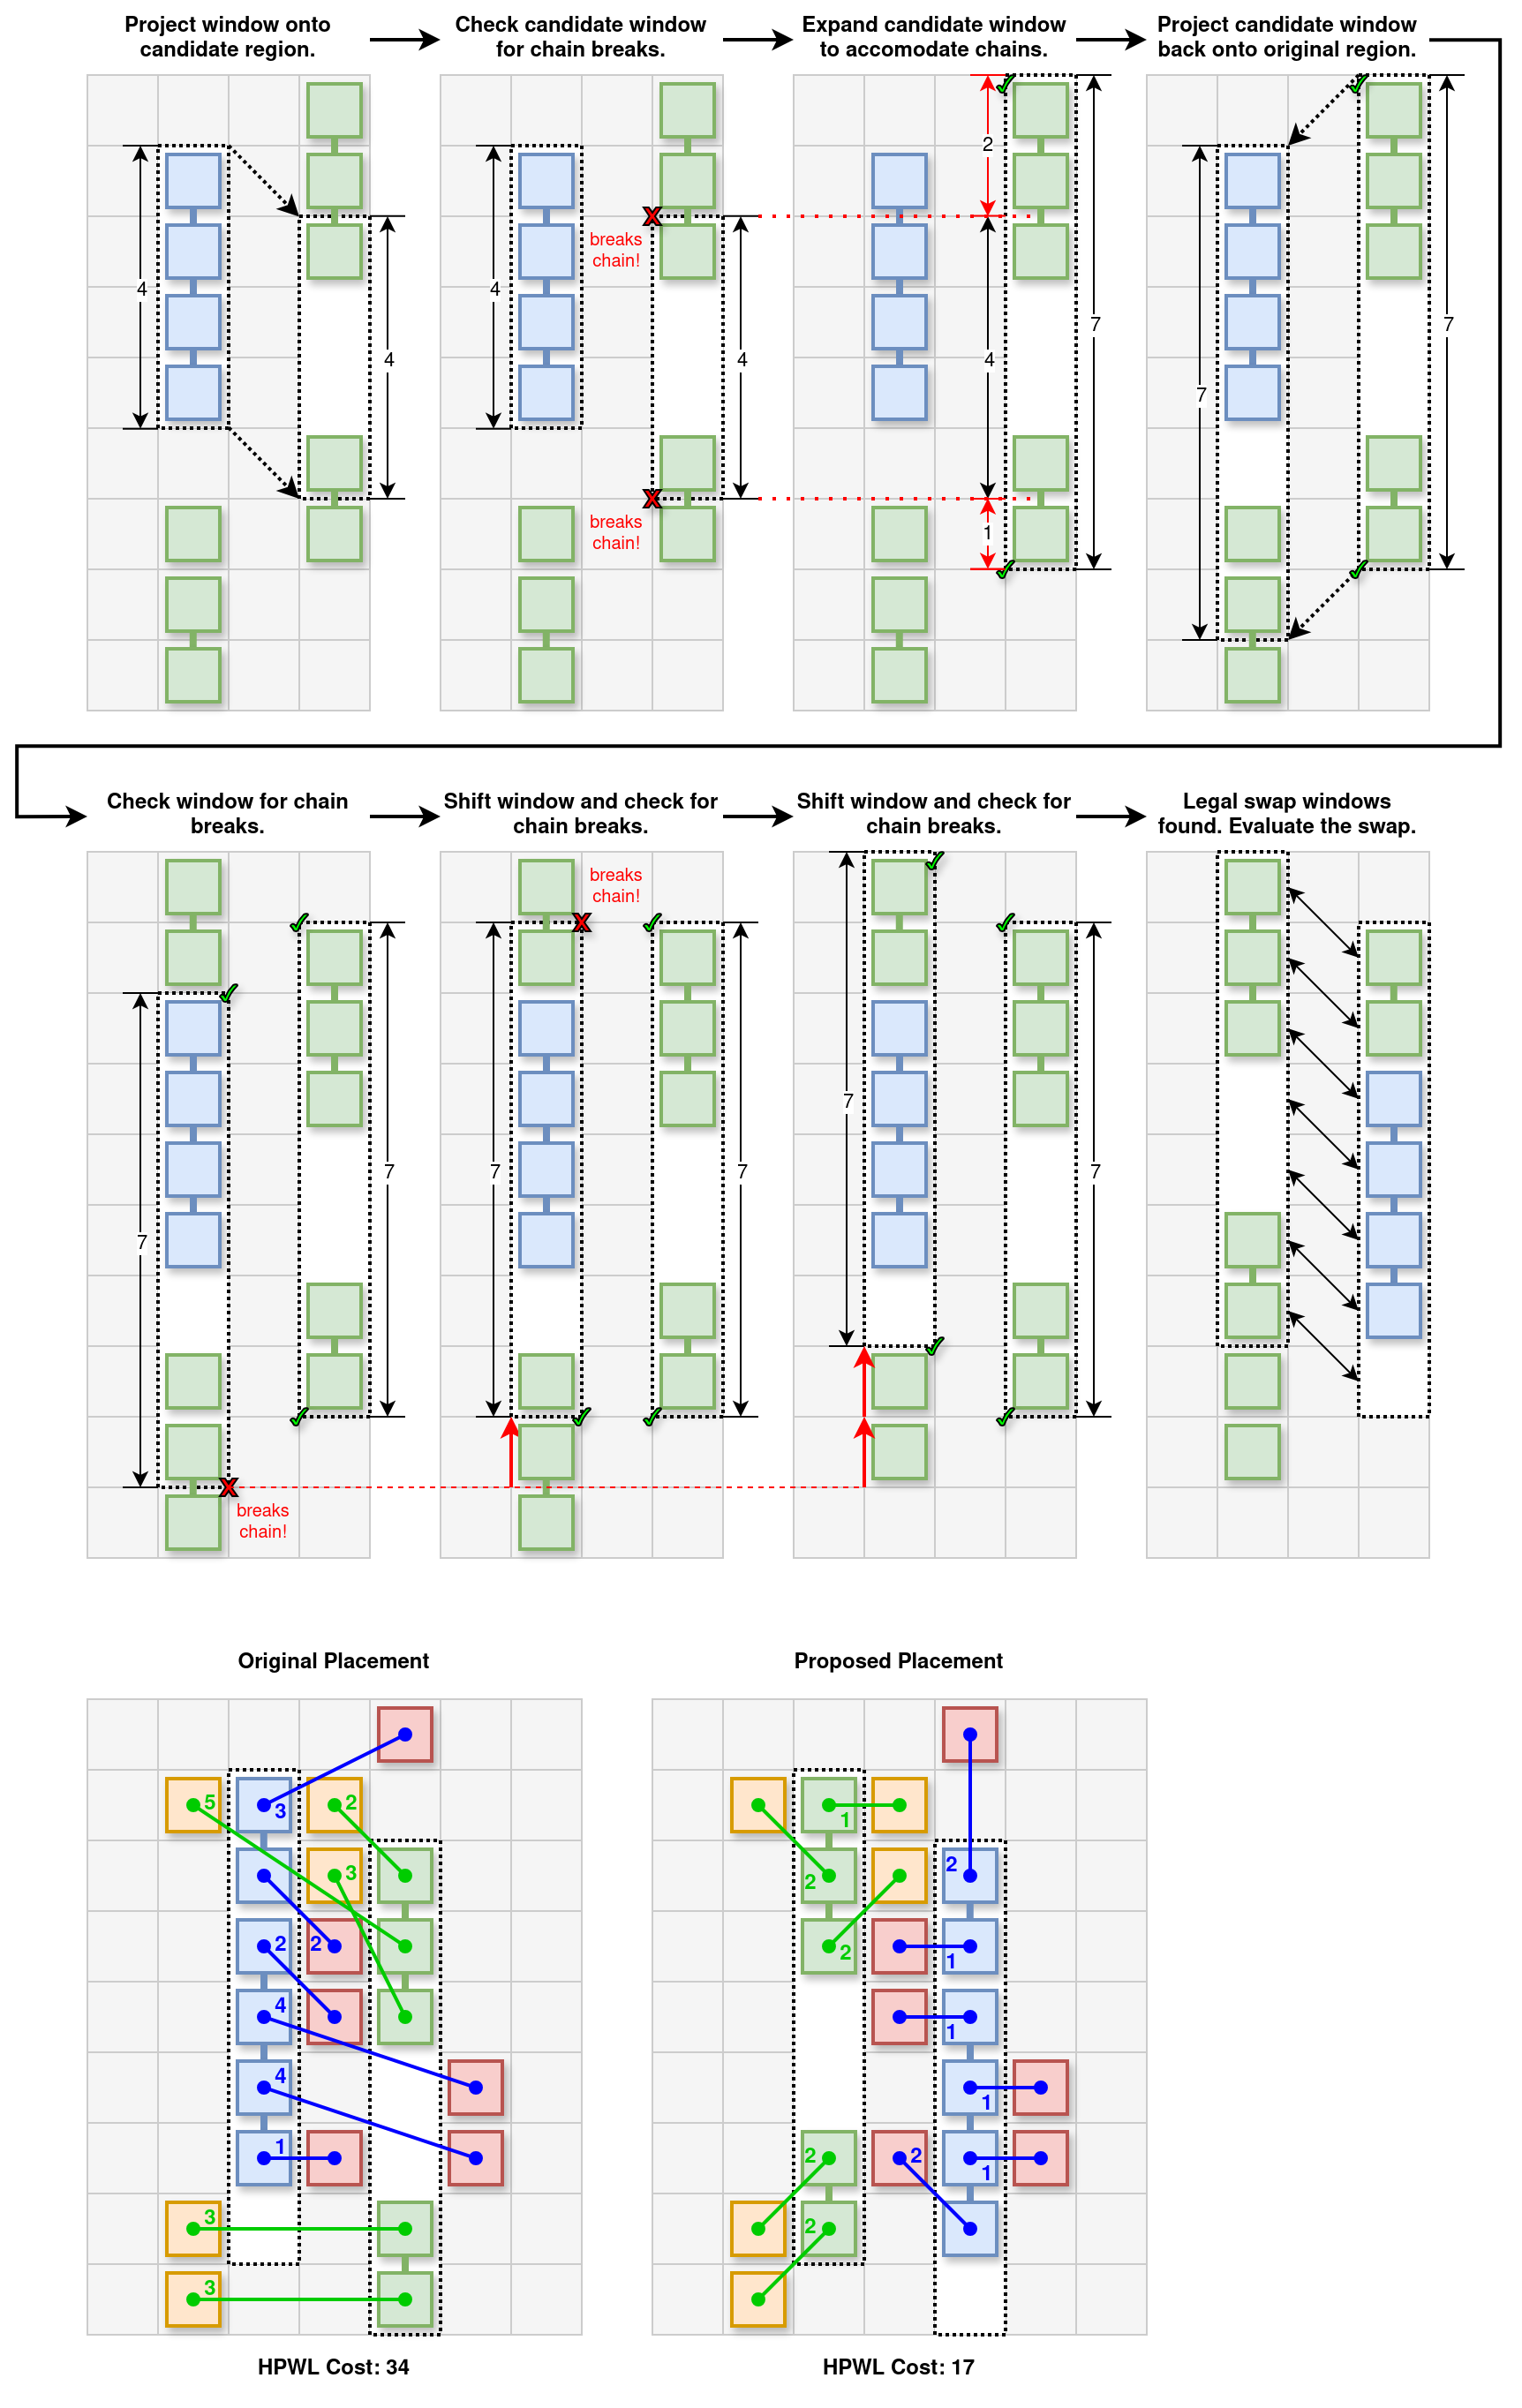
\includegraphics[width=0.9\columnwidth]{figures/placement/swapSiteChain.png}
    \captionof{figure}{Site Chain Swap Proposal}
    \label{fig:swapSiteChain}
}
\begin{multicols}{2}


